\documentclass[
    paper=a4,
    DIV14,
    fontsize=12pt,
    pagesize=pdftex,
    toc=bibliographynumbered
]{scrartcl}
\usepackage[utf8]{inputenc}
\usepackage[T1]{fontenc}
\usepackage[ngerman]{babel}
% \enquote{..} für automatische Anführungszeichen
\usepackage[autostyle=true]{csquotes}
% zusätzliche Optionen für Aufzählumgebungen itemize, enumerate, ..
\usepackage{enumitem}
% mathematische Symbole und Umgebungen
\usepackage{mathtools, amsfonts, amssymb, amsthm}

% Fonts
\usepackage{lmodern}
\usepackage{dsfont}

% Aussehen von Figuren
\usepackage[%
    font=footnotesize,
    margin=0.2em,
    labelfont=bf,
    format=plain,
    labelsep=period
]{caption}
% Ermöglicht Anordnen von Unterfiguren
\usepackage[%
    font=footnotesize,
    margin=0.2em,
    labelfont=bf,
    format=plain,
    labelsep=space
]{subcaption}

% Ermögliche Hyperlinks und anklickbare Referenzen
\usepackage{hyperref}

% stelle Fonts auf Serif
\setkomafont{sectioning}{\rmfamily\bfseries\boldmath}
\setkomafont{descriptionlabel}{\rmfamily\bfseries}
\numberwithin{figure}{section}
\numberwithin{equation}{section}
\numberwithin{table}{section}

% Mengen, wahrscheinlich nicht notwendig
\newcommand*\setZ{\mathds{Z}}
\newcommand*\setR{\mathds{R}}
\newcommand*\setN{\mathds{N}}
\newcommand*\setK{\mathds{K}}

% nummeriere besimmte Gleichungen
\newcommand\numberthis{\addtocounter{equation}{1}\tag{\theequation}}

% Matrizen, Vektoren
\newcommand*\vecz[2]{\begin{pmatrix} #1 \\ #2 \end{pmatrix}}
\newcommand*\vecd[3]{\begin{pmatrix} #1 \\ #2 \\ #3 \end{pmatrix}}
\newcommand*\vecf[4]{\begin{pmatrix} #1 \\ #2 \\ #3 \\ #4 \end{pmatrix}}
\newcommand*\matDD[4]{\begin{pmatrix} #1 & #2 \\ #3 & #4 \end{pmatrix}}

% Titel etc.
\title{Immer der Sonn' entgegen}
\subtitle{Proseminar: Mathematische Modellierung}
\author{Dominik Bendle \and Melissa Hasel \and Thomas Hofmann}
\date{Wintersemester 2016/17}

\begin{document}
\begin{titlepage}
    \maketitle
    \thispagestyle{empty}
    \centering
    \vfill
    % hier passendes Bild einfügen
    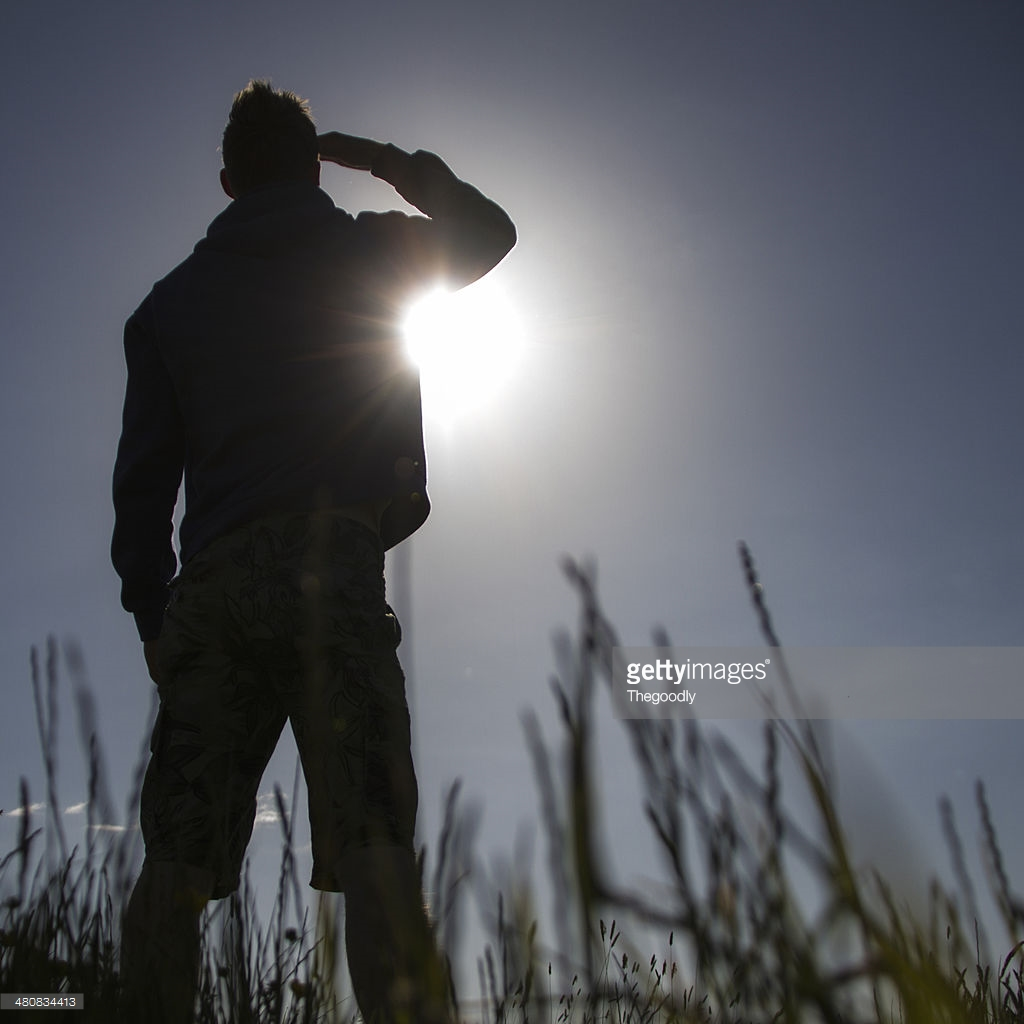
\includegraphics[width=0.7\textwidth]{images/man_looking_at_sun.jpg}
    \vfill
\end{titlepage}

% zweite Seite für Inhalts- und Abbildungsverzeichnis
\tableofcontents
\newpage
\listoffigures
\newpage
\pagestyle{headings}

\section{Problembeschreibung}
Wir beschäftigen uns mit der in folgender Erzählung aufkommender Problemstellung:
\blockquote{
    Peter rüttelte herrscherlich sein Gabelzepter über die Flämmchen, die sogleich gefällig
    zischelnd höher wucherten; stieß die Zinken in den Boden; drapierte die verschränkten
    Arme dicker auf den Stiel, und erkundigte sich tiefsinnig:

    \textit{Wo käm' man da eigentlich hin? Wenn man immerfort \enquote{Der Sonn' entgegen}
    ginge?}

    \textit{Von morgens an? Na, da würd's'De abends wieder am Ausgangspunkt sein},
    entschied ich, voreilig wie immer \dots

    \textit{Nein. Neinein}, sagte er: \textit{Davon kann gar keine Rede sein, daß man
    abends wieder am Ausgangspunkt wäre. Das ist sogar eine ziemlich komplizierte
    Angelegenheit. Zuerst ginge man nach Osten. Dann nach Süden ausholen. Dann, im Laufe
    des Nachmittags, Süd-West…und schließlich nach Westen: immer der Sonn' entgegen.}

    \textit{Am einfachsten wäre's, man führte das Experiment einmal praktisch durch.}

    \textit{Wie, zum Beispiel, der Sonn' entgegen zu gehen. Ich sag' Dir bloß das Eine:
    wenn ich unterwegs an einem Strunk eine KIEFERNGLUCKE erblicken sollte: die wird
    geerntet!}

    \textit{Kannst Du Dir nicht Sparassis ramosa merken, Peter?} tadelte Fritz:
    \textit{Eine Unterbrechung kommt selbstverständlich überhaupt nicht infrage. Und wenn
    uns ein ganzer Harem verlockend in den Weg tänzelte!}
}
Konkret wollen wir also bei gegebenem Startpunkt und -datum bestimmen, welche Route
entsteht, wenn wir von Sonnenauf- bis Sonnenuntergang immer der Sonne  hinterherlaufen
oder -wandern.

% Dieser Teil könnte in den nächsten Abschnitt verschoben werden
Dabei müssen wir die realen Gegebenheiten unserer Umwelt beachten:
Behinderungen jeder Art wie Wände, Zäune, Flüsse und ähnliches müssen erkannt und wenn
möglich umgangen werden.
Zusätzlich wollen wir zur realistischen Beschreibung einer ganztägigen Wanderung auch
Laufpausen erlauben und müssen die entsprechenden Auswirkungen auf den Sonnenstand
betrachten.

% Bedarf sicherlich noch einiger Überarbeitung
\section{Übersicht}
Unsere Strategie bei der Modellierung dieser Problemstellung ist es, mit einem möglichst
einfachen, aber nicht zu unrealistischen Modell zu beginnen und dieses anschließend
sukzessive zu erweitern und zu spezialisieren.

Als Ausgangspunkt wählen wir ein vereinfachtes Umlaufmodell, bei welchem sich die Erde
auf einer perfekten Kreisbahn um die Sonne bewegt. Weiterhin nehmen wir an, dass die Erde
eine perfekte Kugel ist. Dies liefert dann bereits eine gute Intuition für die
entstehende Laufroute. Anschließend erweitern wir das Modell um Höhendaten, um
steigungsbedingte Laufgeschwindigkeiten zu ermöglichen. Dabei verwenden wir die frei
verfügbaren Daten der SRTM.

Um nun Hindernisse und dergleichen modellieren und umgehen zu können, brauchen wir
entsprechende Daten. Der freien Zugänglichkeit wegen wählen wir dieser Stelle
OpenStreetMap als Quelle für Straßendaten. Da der sofortige Übergang zu einem
kollisionsbasierten Modell mit freier Beweglichkeit zunächst zu schwer erscheint,
entwerfen wir ein Fortbewegungsmodell auf Grundlage von Straßen und Wegen, was wiederum
erfordert, sich mit Sackgassen und Rundwegen zu beschäftigen.

Als letzten Schritt in unserer Modellierung versuchen wir uns dann an der
\enquote{Querfeldein}-Variante: Wir wollen uns auch außerhalb von Straßen bewegen
können und müssen dafür Hindernisse erkennen und umgehen. Letztendlich ist das Umgehen in
unserem Modell aber nur relativ primitiv umgesetzt. Abschließend machen wir unsere
Ergebnisse in einer benutzerfreundlichen grafischen Oberfläche zugänglich.

Im Anhang werden die dabei entstandenen Dateien aufgelistet und erläutert. Es wird zudem
erklärt, wie diese zu benutzen sind und welche Funktionen und Projekte wir verwendet haben.

Zur technischen Realisierung der hier präsentierten Modelle verwenden wir \textsc{Matlab}.

\section{Ein einfaches Sonnenmodell}
Zur Realisierung unseres Modell ist es elementar notwendig, für einen gegebenen Zeitpunkt
und eine gegebene Position zu bestimmen, wo oder in welcher Richtung sich die Sonne
befindet, um ihr folgen zu können. Als einfache Umsetzung bieten sich für fast alle
populären Programmiersprachen vorgefertigte Bibliotheken oder Funktionen an, die die
Sonnenposition im Himmel als Winkelpaar berechnen.

Stattdessen wollen wir ein einfaches Planetenmodell im $\setR^3$ entwickeln, mithilfe
dessen wir die Position der Sonne und die entsprechende Gehrichtung unter Verwendung
einfacher linearer Algebra bestimmen können. Dabei beziehen wir uns auf reale Daten und
wollen diese in ein einfacheres Modell vereinfachen.

\subsection{Position der Sonne}

Laut verschiedenen Quellen beträgt der Abstand der Erde zur Sonne im Verlauf eines Jahres
zwischen 147{,}1 und 152{,}1~Millionen Kilometern, wir wählen als mittleren Abstand $d_S =
149\,000\,000\,000\,\mathrm m$. Weiterhin sei die Erde als perfekte Kugel mit Radius $r_E
= 6\,372\,000\,\mathrm m$ gegeben, die sich auf ebenen Kreislinie mit Radius $d_S$ in der
$xy$-Ebene unseres Koordinatensystems gegen den Uhrzeigersinn um die Sonne bewegt. Sie
bewege sich dabei mit konstanter Geschwindigkeit und einer Periode von einem
Standard-Jahr, d.\,h.\ $p_S = 365\cdot 1440 \mathrm{min}$.

\begin{figure}[htb]
    \centering
    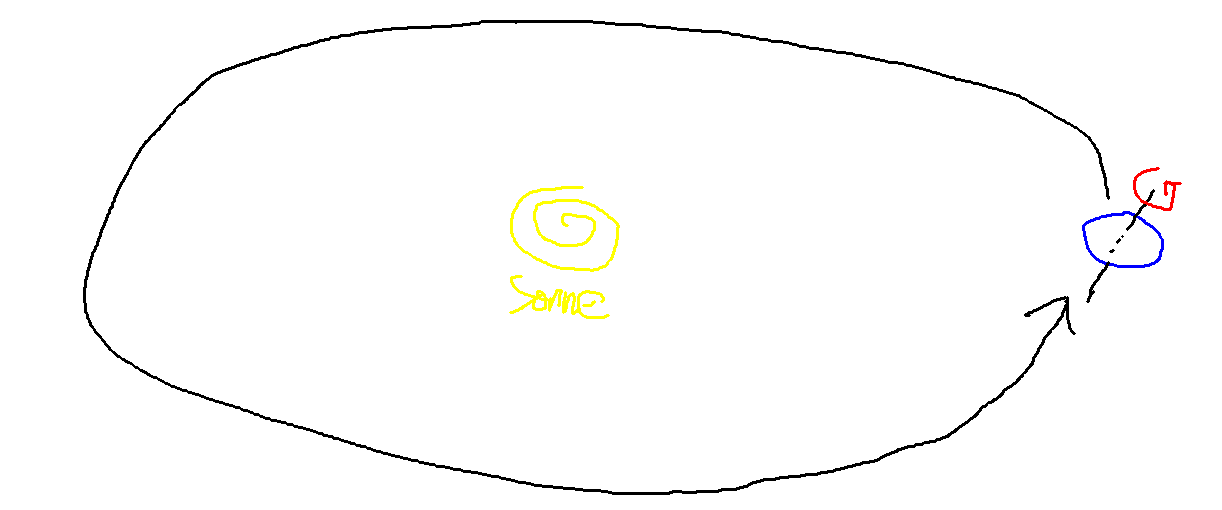
\includegraphics[width=0.95\textwidth]{images/tmp/helioz.png}
    \caption{Heliozentrisches Modell, 21.\ Dezember}
    \label{fig:helioz}
\end{figure}

Bevor wir dies in mathematischen Formeln konkretisieren, ist es sinnvoll, dieses
heliozentrische Modell wie in Abbildung~\ref{fig:helioz} dargestellt in ein geozentrisches
umzuwandeln, da wir im Endeffekt eine fest im Raum stehende Erde betrachten wollen. Sei
dazu die Erde eine im Ursprung zentrierte Kugel mit Radius $r_E$ mit der durch die Gerade
\begin{equation*}
    a : \setR \to \setR^3, t \mapsto t\cdot \vecd{\sin(\alpha_E)}0{\cos(\alpha_E)}
\end{equation*}
gegebenen Rotationsachse, wobei $\alpha_E = 23{,}4^\circ \approx 0{,}13\pi$ die Erdneigung
zur $z$-Achse ist. Die Erde dreht sich hierbei innerhalb eines Tages im Uhrzeigersinn um
die eigene Achse, d.\,h.\ $p_E=1440\,\mathrm{min}$. In diesem geozentrischen Modell soll
die Sonne zum Startzeitpunkt am Punkt $d_S \cdot (1, 0, 0)^T$ über dem Null-Meridian
stehen. Klar ist, dass die Sonne dann am höchsten über der Norhalbkugel steht, also wählen
wir den 21.\ Juni, den Tag der Sommersonnenwende, als Ausgangszeit. Wir messen die Zeit in
Minuten seit dem 1.\ Januar, 0 Uhr UTC, also ergibt sich $t_0=172{,}5 \cdot 1440
\,\mathrm{min}$. Schließlich ergibt sich folgende Parametrisierung für die Sonne im
geozentrischen Modell:
\begin{equation*}
    s: \setR \to \setR^3, t\mapsto d_S \cdot
        \vecd{\cos( \omega(t - t_0) )}{\sin( \omega(t - t_0) )}0
\end{equation*}
wobei $\omega = 2\pi/p_S$. Dieses Modell ist in Abbildung~\ref{fig:geoz} dargestellt.

\begin{figure}[htb]
    \centering
    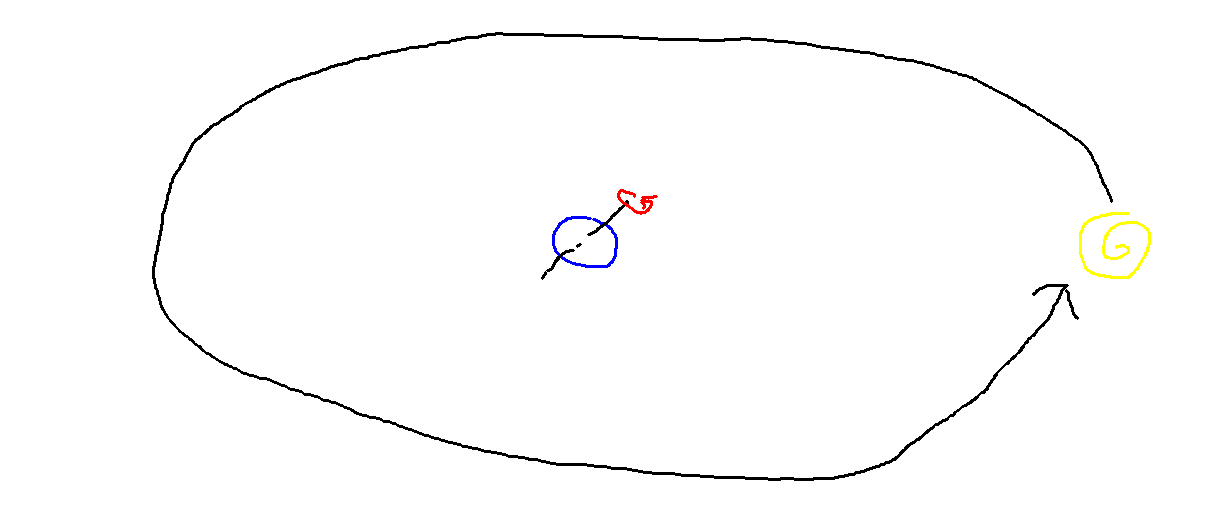
\includegraphics[width=0.95\textwidth]{images/tmp/geoz.png}
    \caption{Geozentrisches Modell, 21.\ Juni}
    \label{fig:geoz}
\end{figure}

In diesem Modell dreht sich die Erde aber um ihre Achse, also sind feste Positionen auf
der Erde nicht fest im Koordinatensystem, was das Arbeiten umständlich macht. Dies
korrigieren wir in zwei Schritten: Zunächst drehen wir das Koordinatensystem so, dass
die Rotationsachse der Erde und die $z$-Achse des Koordinatensystems übereinstimmen und
anschließend kehren wir die Erdrotation um, sodass die Erde zeitunabhängig im
Koordinatensystem sitzt.

Da die Erdrotationsachse in unserem Modell in der $xz$-Ebene liegt, müssen wir das
Koordinatensystem um die $y$-Achse drehen. Eine solche Rotationsmatrix ist für einen
Winkel $\alpha\in\setR$ durch
\begin{equation*}
    R_y(\alpha) =
    \begin{pmatrix}
        \cos(\alpha)  & 0 & \sin(\alpha) \\
        0             & 1 & 0            \\
        -\sin(\alpha) & 0 & \cos(\alpha)
    \end{pmatrix}
\end{equation*}
gegeben, was durch Nachvollziehen der Drehungen der Einheitsvektoren klar wird. Aus
unserer Konstruktion ist nun einfach nachzuvollziehen, dass wir unser Koordinatensystem um
den Winkel $-\alpha_E$ drehen müssen, denn $R_y(-\alpha_E)\cdot a(t) = (0, 0, t)^T$.

Als nächstes wollen wir die Erdrotation -- jetzt um die $z$-Achse -- aufheben. Analog zu
oben ergibt sich eine entsprechende Rotationsmatrix
\begin{equation*}
    R_z(\alpha) =
    \begin{pmatrix}
         \cos(\alpha) & \sin(\alpha) & 0 \\
        -\sin(\alpha) & \cos(\alpha) & 0 \\
        0             & 0            & 1
    \end{pmatrix}
\end{equation*}
für Winkel $\alpha\in\setR$. Um nun die Erde für jeden beliebigen Zeitpunkt $t\in\setR$
auf die Ausgangsposition zu $t_0$ \enquote{zurückzudrehen}, müssen wir offenbar um
$-\omega_E(t-t_0)$ drehen, mit $\omega_E = 2\pi/p_E$. Somit erhalten wir die folgende
Parametrisierung für die Sonne in unserem geozentrischen Modell:
\begin{equation*}
    P_S : \setR \to \setR^3, t\mapsto R_z(-\omega_E(t-t_0)) \cdot R_y(-\alpha_E) \cdot
    s(t),
\end{equation*}
die Veränderungen sind in Abbildung~\ref{fig:geomod} erkennbar. Wir bemerken vorab das
Kugelkoordinaten $(\alpha, \beta, r_E)$ für Punkte $p \in E := \{ x\in\setR^3 \mid \|x\| =
r_E \}$ genau den Koordinaten des entsprechenden Punktes in Längen- und Breitengraden
entsprechen.

\begin{figure}[hbt]
    \centering
    \begin{subfigure}{0.48\textwidth}
        \centering
        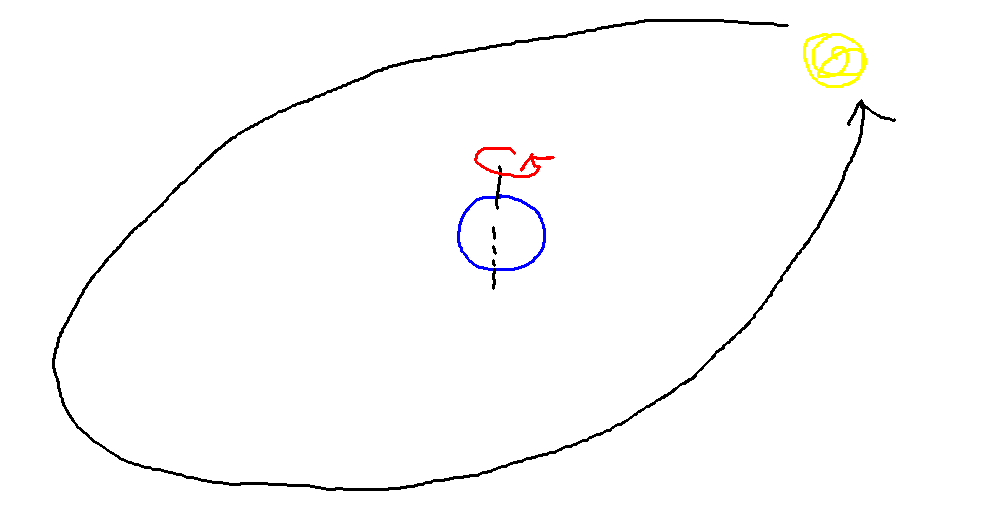
\includegraphics[width=0.98\textwidth]{images/tmp/geomod1.png}
        \caption{mit Erdrotation}
    \end{subfigure}
    \begin{subfigure}{0.48\textwidth}
        \centering
        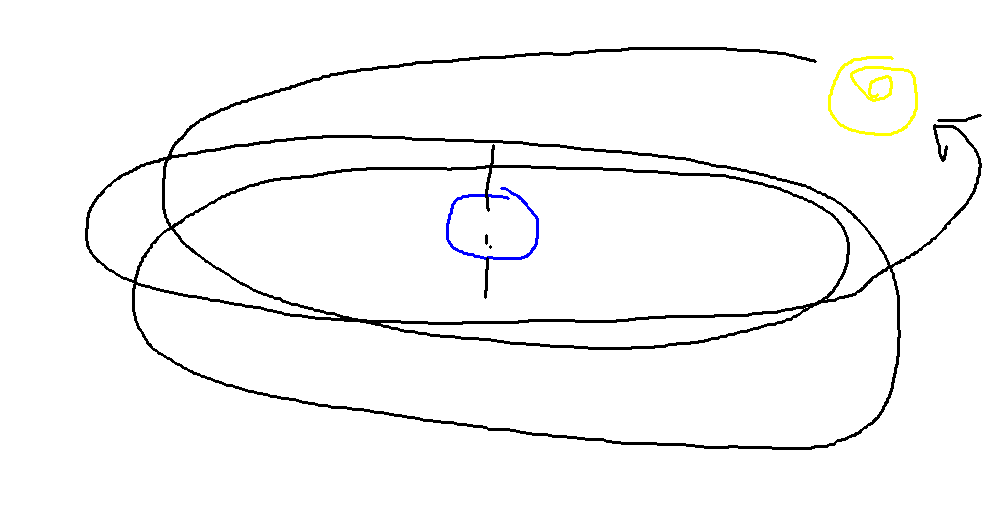
\includegraphics[width=0.98\textwidth]{images/tmp/geomod2.png}
        \caption{Erdrotation korrigiert}
    \end{subfigure}
    \caption{Begradigung der Rotationsachse}
    \label{fig:geomod}
\end{figure}

\subsection{Laufmodell und Richtungsbestimmung}
Mit der Parametrisierung der Sonnenposition lässt sich nun für eine gegebene Position und
Zeit bestimmen, welche die nächste Position in Richtung Sonne ist. Es seien $p_0$ unser
Ausganspunkt und $t$ die Ausgangszeit. Da es sich hierbei um einen diskreten Prozess
handelt, sei $\Delta_t$ die Laufdauer (in min) und $v$ die Laufgeschwindigkeit (in m/min).
Da wir uns zu Fuß fortbewegen, können wir für relativ kleine $\Delta_t$ annehmen, dass die
unmittelbar umgebende Kugeloberfläche eben ist. Um nun die Laufrichtung in Richtung Sonne
zu bestimmen genügt es, den Verbingunsvektor von $p$ nach $P_S(t)$ auf die Tangentialebene
von $E$ in $p$ zu projizieren. Diese Ebene ist durch den normierten Normalenvektor
$n_p = p/\|p\|$ gegeben, sodass sich die Projektion $p_S$ wiefolgt ergibt:
\begin{equation*}
    p_S = \left( P_S(t) - p \right) - \left( (P_S(t) - p)\cdot n_p \right) \cdot
    n_p
\end{equation*}
Um nun die gewünschte Distanz in Richtung Sonne gehen, addieren wir einfach den normierten
Vektor mit geeignetem Faktor:
\begin{equation*}
    \tilde p = p + \frac{v\cdot\Delta_t}{\|p_S\|} p_S.
\end{equation*}
Anschließend müssen wir unsere neue Position durch anpassen der Norm zurück auf die Kugel
projizieren:
\begin{equation}
    p_{\text{neu}} = \frac{r_E}{\|\tilde p\|}\tilde p.
    \label{eq:pneu}
\end{equation}
Mit diesen Berechnungen lässt sich nun iterativ die Laufroute auf einer idealen Erde
berechnen. Wie in Abbildung~\ref{fig:sonnenmodellroute} dargestellt, ergibt sich dabei wie
intuitiv vielleicht erwartet eine elliptische bis kreisförmige Bahn.

\begin{figure}[ht]
    \centering
    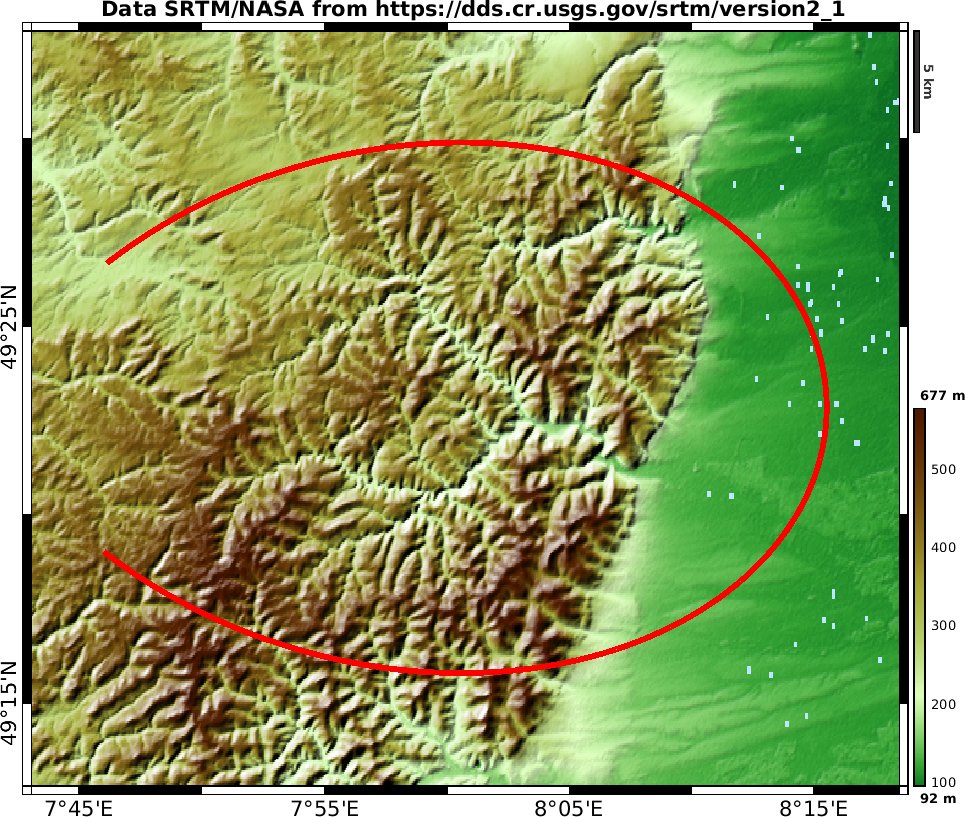
\includegraphics[width=0.7\textwidth]{images/ideal.png}
    \caption{Ideale Laufroute auf topologischer Karte bei Kaiserslautern, 21.\ Juni}
    \label{fig:sonnenmodellroute}
\end{figure}

Schließlich wollen wir noch prüfen, wann die Sonne nicht mehr sichtbar -- also
untergegangen -- ist, um unsere Berechnungen sinnvoll terminieren lassen zu können.
Im wesentlichen müssen wir dafür den Winkel zwischen der Blickrichtung gen Sonne
$P_S(t) - p$ und dem Normalenvektor $n_p$ bestimmen. Für Vektoren $a, b\in \setR^3$ gilt
dabei
\begin{equation*}
    a\times b = \|a\|\|b\| \sin \alpha \cdot n \qquad
    a \cdot b = \|a\|\|b\| \cos \alpha
\end{equation*}
für $\alpha = \measuredangle(a, b)$. Daraus folgt dann $\tan\alpha = \|a\times b\|/(a\cdot
b)$. Da der Tangens nicht bijektiv ist, müssen wir den Winkel über $\alpha =
\mathrm{atan2}(\|a\times b\|, a\cdot b)$ berechnen. Nun ist nur noch zu entscheiden, für
welche Winkel die Sonne nicht mehr sichtbar ist: Eine naheliegende und einfache Annahme
ist, für $\measuredangle(P_S(t) - p, n_p) > 90^\circ$ nichts zu tun.

Mithilfe dieser Information können wir auch für gegebene Position und Zeit den den
nächsten oder letzten Sonnenauf- und Untergang bestimmen, indem wir einfach mit kleinem
$\Delta_t$ vor- oder zurückzählen, bis die Sonne auf- oder untergeht. Dies verwenden wir
später, wenn wir in unserem Modell bei Sonnenaufgang beginnen wollen.

\subsection{Vergleich mit exakten Berechnungen}
Nach Entwurf dieses Modells stellt sich selbstverständlich die Frage, wie realistisch es
nach all den Vereinfachungen noch ist. Der Einfachheit halber verwenden hier zum Vergleich
eine vorgefertigte Funktion zur Berechnung der Sonnenposition, anstatt entsprechende
Algorithmen selbst zu implementieren.

\begin{figure}[hbt]
    \centering
    \begin{subfigure}{0.47\textwidth}
        \centering
        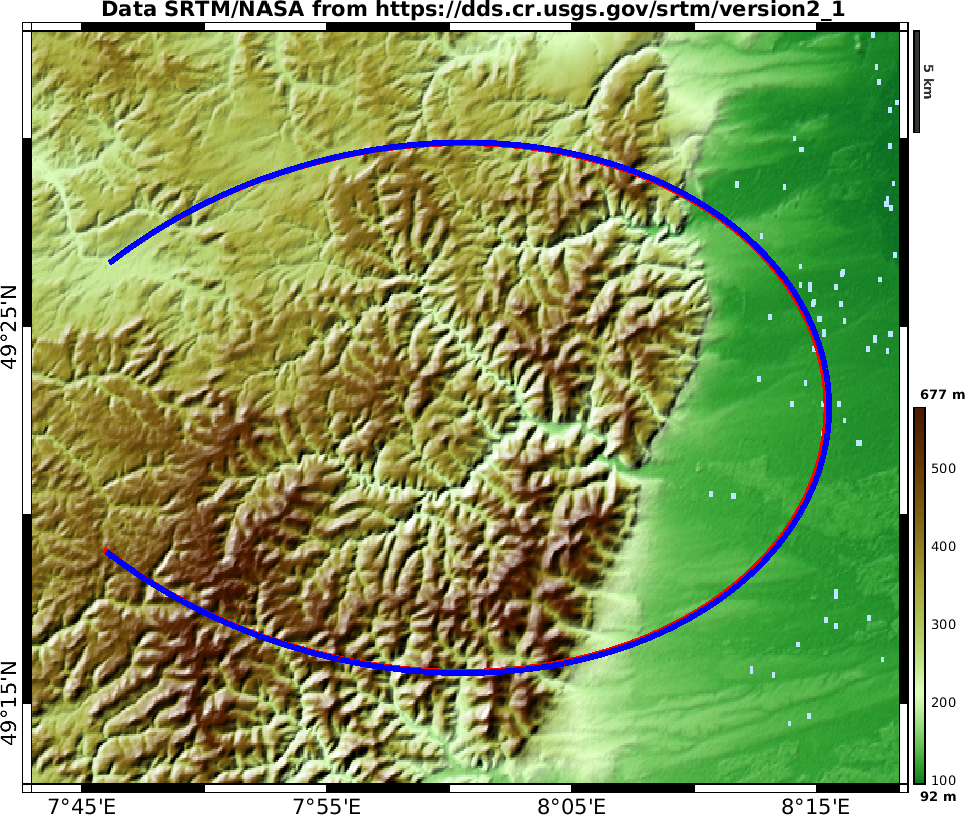
\includegraphics[width=0.98\textwidth]{images/sunposdiffideal.png}
        \caption{im idealen Laufmodell}
    \end{subfigure}
    \begin{subfigure}{0.51\textwidth}
        \centering
        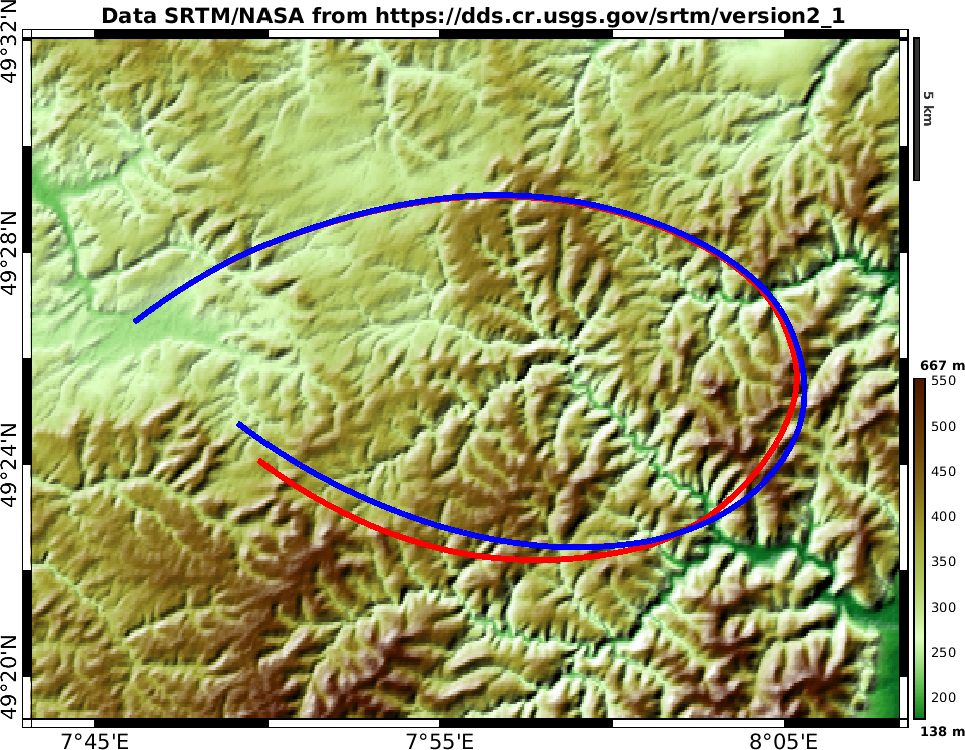
\includegraphics[width=0.98\textwidth]{images/sunposdiffele.png}
        \caption{Mit Höhendaten, siehe nächsten Abschnitt}
    \end{subfigure}
    \caption{Startpunkt bei Kaiserslautern (blau unseres, rot exaktes Modell)}
    \label{fig:sunposmoddiff}
\end{figure}

Erkennbar ist nun in Abbildung~\ref{fig:sunposmoddiff}, dass im idealen Laufmodell kaum
Unterschiede existieren, erweitern wir das Modell wie im nächsten Abschnitt jedoch um
zusätzliche Information, so kann diese bei kleinen Positionsdifferenzen zu größerer
Divergenz der Routen führen.

\subsection{Laufpausen}
Bevor wir mit der Erweiterung des Modells fortfahren, wollen wir noch anmerken, dass es
eher unrealistisch ist, einen ganzen Tag lang ununterbrochen durchzulaufen. Aus diesem
Grund fügen wir unserem Modell die Möglichkeit hinzu, Pausen einzulegen. Wir setzen dies
jedoch statisch und benutzerdefinierbar um, da sich keine guten allgemeingültigen Aussagen
über das Laufverhalten verschiedener Benutzer machen lässt.

\section{Erweiterung um Höhendaten}
Eine naheliegende nächste Erweiterung des Modells ist das Einbeziehen von Höhendaten, um
entsprechend die Laufgeschwindigkeit in zum Beispiel hügligerem Gelände zu beschreiben.

\subsection{Höhendaten und Laufgeschwindigkeit}
% Erwähne früher im Text, dass Matlab benutzt wird
Als Quelle der Höhendaten wählen wir die seit 2015 frei verfügbaren Daten der
internationalen SRTM (Shuttle Radar Topography Mission). Der Zugriff auf diese Daten wird
uns durch ein durch einen Matlab-Nutzer vorgefertigtes Skript erleichtert, sodass an
dieser Stelle wenig Implementierungsaufwand entsteht.

Die von der SRTM bereitgestellten Daten liefern Höhendaten zu Koordinaten zwischen
60$^\circ$ nördlicher Breite und 59$^\circ$ südlicher Breite, wobei der Abstand zwischen
Datenpunkten von 30 bis 90 Meter reicht. Dies ist zwar gerade im Kontext der etwas
langsameren Bewegung zu Fuß nicht sehr genau, für mittlere Steigungen sind die Daten aber
mehr als ausreichend.

Unter Verwendung linearer Interpolation können wir nun von der Existenz einer
Höhenfunktion $e : [-180^\circ, 180^\circ]\times[-59^\circ, 60^\circ] \to \setR$ ausgehen,
die wir zur Bestimmung mittlerer Steigungen verwenden können. Also müssen wir die
Auswirkung der Steigung auf die Laufgeschwindigkeit untersuchen: Eine mögliche
Beschreibung dieser Beziehung ist Toblers Hiking-Funktion \cite{wp:tobler}, die wie folgt
definiert ist:
\begin{equation*}
    v = 6e^{-\left| \frac{\Delta e}{\Delta x} + 0{,}05 \right|}
\end{equation*}
mit Geschwindigkeit $v$ in km/h, Höhendifferenz $\Delta e$ und Distanz $\Delta x$, wobei
die Funktion eine Höchstgeschwindigkeit von 6\,km/h ausgibt -- das beschrieben Verhältnis
von Steigung zu Laufgeschwindigkeit ist in Abbildung~\ref{fig:tobler} abgebildet. Es seien
nun $v_{\text{max}}$ die maximale Geschwindigkeit in m/min, $\Delta_t$ die zu laufende
Zeit, $p$ unser Ausgangspunkt und $p_{\text{neu}}$ die wie in \eqref{eq:pneu} bestimmte
nächste Position. Zudem soll die Funktion kart2sph kartesische Koordinaten in ein
Tupel\footnote{Die Länge des Vektors ist uninteressant.} der entsprechenden
Kugelkoordinaten konvertieren. Dann definiere
\begin{equation}
    v_{\text{Tobler}} = v_{\text{max}} \cdot \exp\left|
    \frac{e(\mathrm{kart2sph}(p_\text{neu})) - e(\mathrm{sph2kart}(p))}{v_{\text{max}}
    \cdot \Delta_t} + 0{,}05 \right|
    \label{eq:tobler}
\end{equation}
Die Idee ist nun, immer die konstante vertikale Distanz von $v_{\text{max}}\cdot\Delta_t$
zurückzulegen und die passende Zeit $\Delta_t \cdot v_{\text{max}} / v_{\text{Tobler}}$
verstreichen zu lassen.

\begin{figure}[htb]
    \centering
    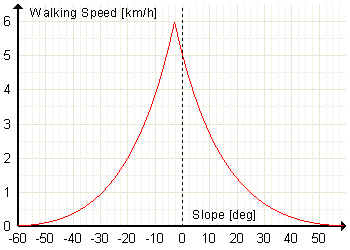
\includegraphics[width=0.5\textwidth]{images/tobler.png}
    \caption{Toblers Hinkingfunktion, Quelle: Wikimedia, \cite{wp:tobler}}
    \label{fig:tobler}
\end{figure}

\subsection{Vergleich zum vorigen Modell}
Nun stellt sich die Frage, ob der Einbezug der Höhendaten einen wesentlichen Effekt auf
die Laufroute hat. Da sich auf keine offensichtliche Art und Weise mathematisch prüfen
lässt, wollen wir einige Beispiele betrachten.

In Abbildung~\ref{fig:elediff1} starten wir mit den Koordinaten $(7{,}768889^\circ,
49{,}444722^\circ)$, was bei Kaiserslautern liegt, und können einen wesentlichen Unterschied im
Verlauf der Route feststellen. Das in den topografischen Karten erkennbare hügelige
Terrain sorgt dafür, dass wir unter Berücksichtigung der Höhendaten im Mittel sehr viel
langsamer laufen und somit einen kleineren Bereich mit unserer Laufroute abdecken.
Weiterhin ist in (b) auch zu sehen, dass die elliptische Form verloren geht, da die
Laufgeschindigkeit größeren Schwankungen unterliegt.

\begin{figure}[hbt]
    \centering
    \begin{subfigure}{0.31\textwidth}
        \centering
        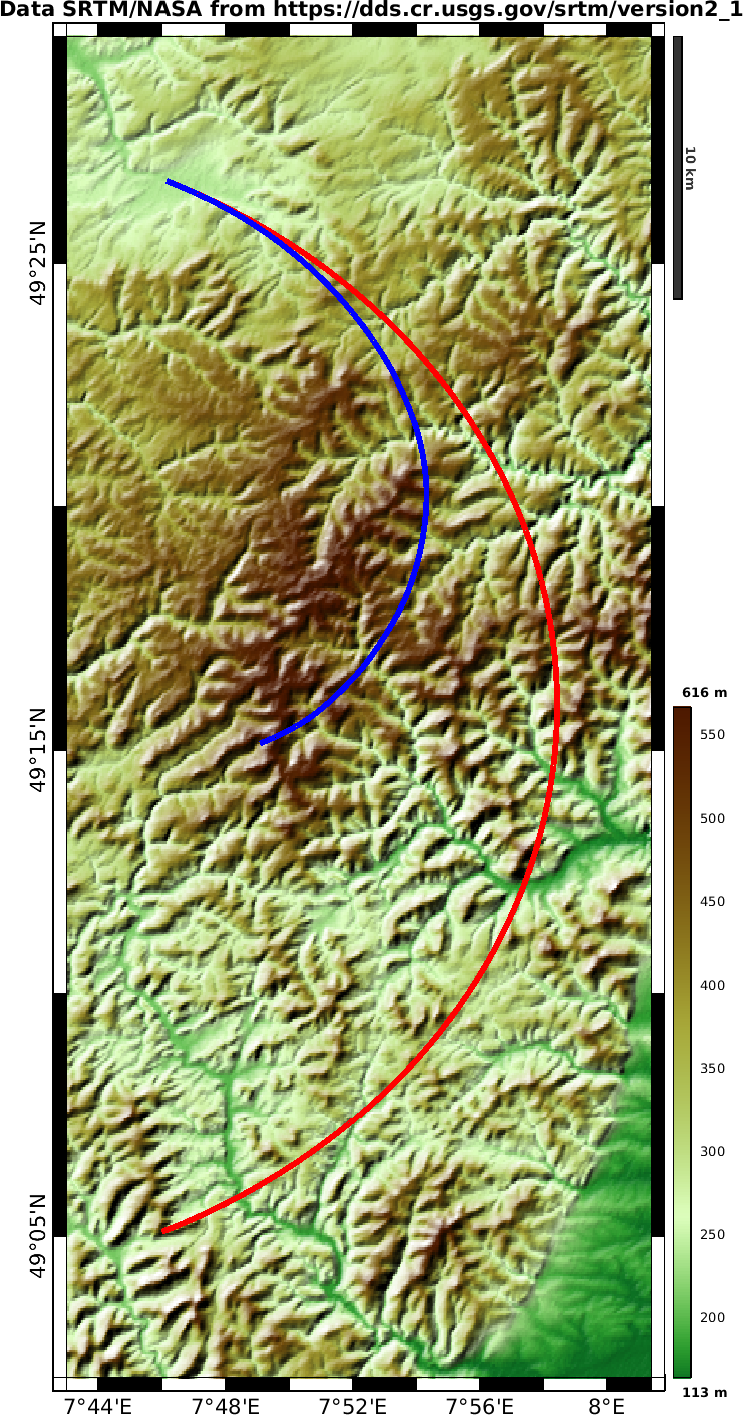
\includegraphics[width=0.98\textwidth]{images/elediff/feb13.png}
        \caption{13.\ Februar}
    \end{subfigure}
    \begin{subfigure}{0.67\textwidth}
        \centering
        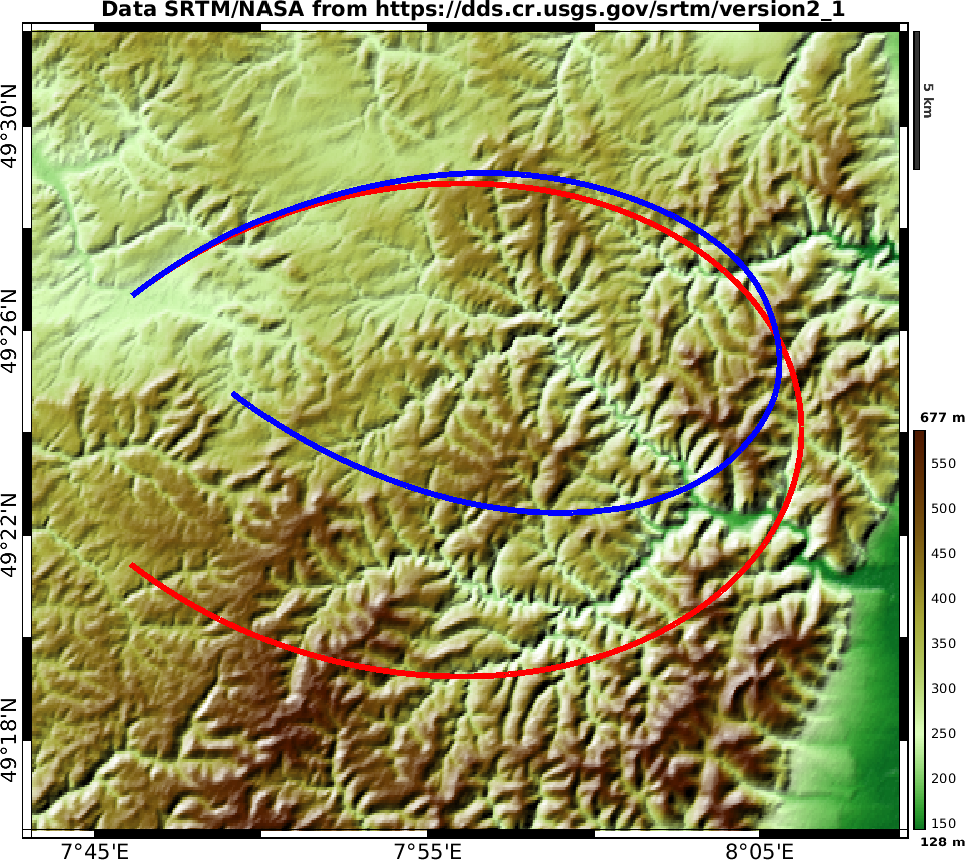
\includegraphics[width=0.98\textwidth]{images/elediff/jun21.png}
        \caption{21.\ Juni}
    \end{subfigure}
    \caption{Startpunkt bei Kaiserslautern (blau mit, rot ohne Höhendaten) bei gleicher
    Durchschnittsgeschwindigkeit.}
    \label{fig:elediff1}
\end{figure}

Somit ist zumindest ersichtlich, dass das Modell durch Hinzunahme von Höhendaten und
variabler Laufgeschwindigkeit wesentlich beeinflusst wird. Wir müssen hier natürlich
annehmen, dass die Hikingfunktion eine gute Beschreibung der Realität liefert, was aber
für gröbere Schätzungen gewährleistet ist.

\section{Realitätsbasierte Daten: OpenStreetMap}
Für alle weiteren von uns als sinnvoll erachteten Erweiterungen des Modells ist es
notwendig, Karten- oder Straßendaten einzubeziehen. Wir wählen hierfür den
OpenStreetMap-Dienst, da er API-Zugriffe auf Kartendaten ohne besondere Accounts oder
Entwicklerschlüssel zulässt und weiterhin auch gut dokumentiert ist.

Ein Großteil unserer Projektarbeit hat sich damit beschäftigt, wie wir mit den
OpenStreetMap kommunizieren und die erhaltenen Dateien verarbeiten können. Im Wesentlichen
verwenden wir eine \textsc{Matlab}-Funktion, die OpenStreetMap-Daten aus dem XML-Format in
ein leicht verwendbares Struct umwandelt. Diese Daten müssen dann über API-Anfragen an die
entsprechenden Server angefordert werden.
% mehr?

\subsection{Bewegung auf Grundlage von Straßen und Wegen}
In unserem ersten Erweiterungsversuch um Kartendaten haben wir unseren Fokus auf Straßen
und befestigte Wege gelenkt, auf denen wir uns bewegen wollen. Hierbei entstehen zwei
Problemstellungen:
\begin{enumerate}[label=\arabic*.,leftmargin=1.5em]
    \item Wie in zum Beispiel Abbildung~\ref{fig:sunposmoddiff} erkennbar überbrücken wir
        große Distanzen bei einem eintägigen Lauf. Das gesamte umschließende Rechteck als
        Karte hat meist eine Größe mehrerer hundert Megabyte kann nur mit enormem
        Zeitaufwand verwendet werden.

        In unserem Ansatz zentrieren wir ein kleines Koordinatenrechteck um unsere
        Ausgangsposition und bewegen uns, bis wir an die Grenze des Rechtecks stoßen. Dann
        zentrieren wir das Rechteck neu und laden die Kartendaten neu herunter. Dieser
        Ansatz stellt sich als recht performant heraus.
    \item Wir müssen uns überlegen, nach welchen Kriterien wir uns entlang der Straßen und
        Wege bewegen, da die Position der Sonne gegebenenfalls nicht immer zur Bestimmung
        der nächsten Position ausreicht. Dies wollen wir in den nächsten Absätzen prüfen.
\end{enumerate}
Wir speichern das unserem Wegmodell zugrundeliegende Straßen- und Wegnetzwerk als
Adjazenzmatrix, um einfach adjazente Knoten ermitteln zu können. Weiterhin merken wir uns
während dem Laufen den zuletzt besuchten Knoten und die bisher gelaufene Distanz. Wir
modellieren die Straßennavigation wie folgt, wobei wir Terminologie aus der Graphentheorie
für den das Straßennetz darstellenden Graphen verwenden:
\begin{enumerate}[label=(\alph*),leftmargin=2em]
    \item Haben wir nur einen Nachbarn, so befinden wir uns am Ende einer Sackgasse. Wir
        vermerken, dass wir uns in einer Sackgasse befinden und bewegen uns zurück zum
        einzig verfügbaren Nachbarknoten.
    \item Haben wir abzüglich unseres Vorgängers nur einen Nachbarknoten, so befinden wir
        uns auf einem Straßensegment, das keine Kreuzung ist. Damit wir bei ungünstiger
        Sonnenposition nicht steckenbleiben bewegen wir uns zum Nichtvorgängerknoten. Auf
        diese Weise laufen wir eine Straße immer komplett ab und entscheiden unser
        Laufverhalten nur an Kreuzungen. Dies verhindert auch das Steckenbleiben in
        Sackgassen.
    \item Haben wir abzüglich unseres Vorgängers mehr als einen Nachbarknoten, so befinden
        wir uns an einer Kreuzung. Es sind nun mehrere Dinge zu erledigen:
        \begin{enumerate}[label=(\roman*)]
            \item Ist die derzeitige \enquote{Herkunftsstraße} wie in (a) markiert eine
                Sackgasse, so markiere den Vorgängerknoten als Sackgasseneingang.
            \item Streiche alle bekannten Sackgasseneingänge aus der Liste der adjazenten
                Knoten, um deren Wiederbesuch zu verhindern. Streiche weiterhin den
                Vorgänger aus der Liste, um nicht kehrt machen zu müssen.
                \label{enum:streichsackg}
            \item Es seien die verbleibenden Nachbarn als $p_i \in \setR^3$ gegeben,
                unsere Position sei $p\in\setR^3$, dann bestimme den Index $i$, sodass
                $(p_i - p) \cdot (P(t) - p)$ maximal ist: Mit dem Skalarprodukt überprüfen
                wir, welche Gangrichtung am besten mit der Sonnenrichtung übereinstimmt.
                Diese wird dann als nächste Position gewählt.
        \end{enumerate}
        \label{enum:kreuz}
\end{enumerate}
Zur Berechnung der dabei verstreichenden Zeit können wir wieder \eqref{eq:tobler}
verwenden, wobei wir die Distanz $v_{\text{max}}\cdot\Delta_t$ durch die tatsächliche
Distanz zwischen den besuchten Knoten ersetzen.

\begin{figure}[htb]
    \centering
    % evtl. zu hochauflösend
    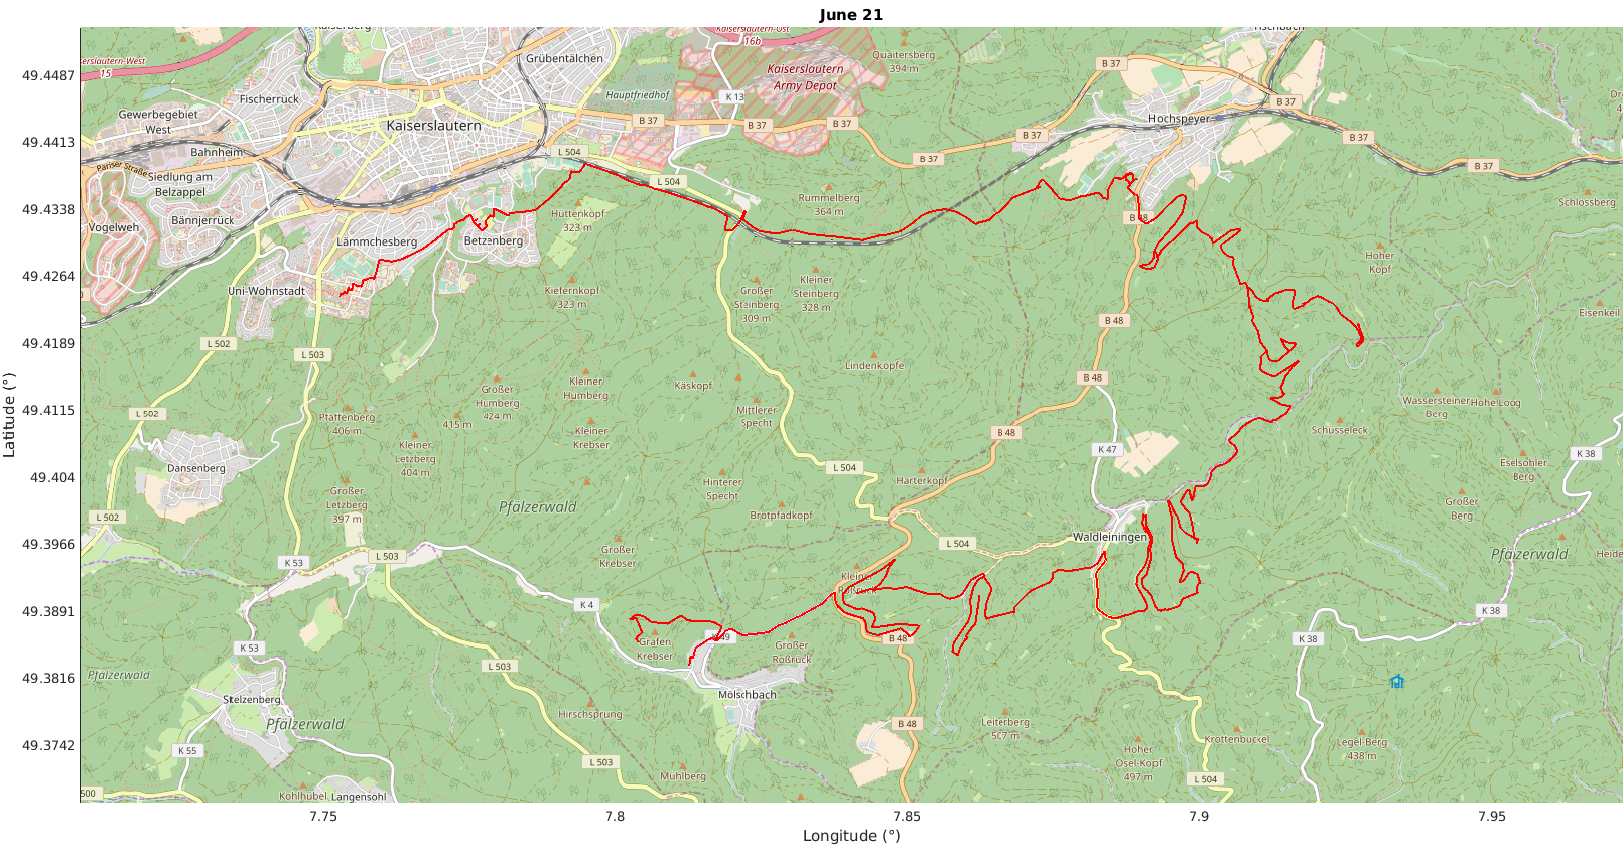
\includegraphics[width=0.98\textwidth]{images/tukl_strasse_gross.png}
    \caption{Das Straßenmodell in Aktion}
    \label{fig:osmmod}
\end{figure}

Mit diesem Vorgehen erzielen wir bereits gute Ergebnisse, aber in bestimmten
Konfigurationen laufen wir uns ein Zykeln im Straßennetztwerk fest, bis sich die
Sonnenposition genügend geändert hat. Die naheliegende Lösung ist nun, alle besuchten
Knoten zu vermerken, um an wiederbesuchten Kreuzungen nicht immer die gleiche Entscheidung
zu treffen. Es sei also $i$ die Anzahl der besuchten Knoten bzw.\ der gemachten
Berechnungsschritte und $K$ die Menge der Knoten\footnote{OpenStreetMap gibt einen
eindeutigen Schlüssel für jeden Knoten vor.}, dann sei $N:\{1, \dots, i\} \to K$ die Folge
der von uns besuchten Knoten. Befinden wir uns im obigen Fall \ref{enum:kreuz}, so
definiere
\begin{equation*}
    I = \bigl\{ \ell \in \{1, \dots, i-1\} \mid
    N(\ell) = N(i) \wedge N(\ell-1) = N(i-1) \bigr\},
\end{equation*}
die Menge der Schritte in denen wir uns bereits an der jetzigen Kreuzung befanden und aus
der gleichen Richtung kamen. Nun füge diesen Schritt nach obigem \ref{enum:streichsackg}
ein: Solange $I\neq\varnothing$ und mindestens zwei Nachbarn übrig sind, entferne $\max I$
aus den Nachbarn und aus $I$. Auf diese Weise werden die als letztes getroffenen
Entscheidungen zuerst ausgeschlossen.

\begin{figure}[htb]
    \centering
    PLATZHALTER FÜR ZYKEL-BEISPIEL
    \caption{Kreislaufen im Straßenmodell}
    \label{fig:osmzyk}
\end{figure}

\subsection{Verallgemeinerung auf straßenloses Modell}

Dies ist ein Beispielsatz.

\section{Integration der Modelle in eine grafische Oberfläche}

Um den Nutzer ein möglichst einfaches und intuitives Nutzen des Programms zu ermöglichen,
werden alle Funktionsaufrufe von der Grafische Benutzeroberfläche (GUI) aus gesteuert,
zu sehen in Abbildung~\ref{fig:GUI}.

Im Zentrum befindet sich das dynamische Koordinatensystem, welches unmittelbar nach dem
Ausführen noch leer ist und später den aktuellen Kartenausschnitt anzeigt. Im Unteren
Bereich finden sich Felder für die Eingabe des Datums, der Geschwindigkeit,
Laufen-Pause-Intervalle und der Koordinaten. Neben der manuellen Eingabe der Koordinaten,
besteht ebenso die Möglichkeit durch klicken der Maustasten einen Koordinatenpunkt auf der
Weltkarte auszuwählen. Um zwischen diesen Möglichkeiten zu wechseln, ist eine Checkbox
über den Koordinatenfeldern platziert.

In der rechten unteren Ecke befindet sich der \enquote{Los}-Button zum Errechnen der Route
und darüber der Button zum Animieren der Route.

In der linken oberen Ecke befindet sich unter dem Namen des Programms die Menüleiste. Es
stehen die Punkte \enquote{Allgemein}, \enquote{Zoom-Modus} und \enquote{Beispiele} zur
Auswahl. Im Reiter Allgemein kann man zwischen den beiden Modi \enquote{entlang der
Straßen} und \enquote{Querfeldein} hin und her wechseln, die einzelnen heruntergeladenen
Kartendaten löschen und das Programm beenden. Im zweiten Reiter Zoom-Modus kann man den
Karten-Zoom aktivieren oder den Zoom zurücksetzen. Im dritten Reiter Beispiele kann man
Beispiele laden, zurücksetzen, speichern und löschen.

\begin{figure}[htb]
    \centering
    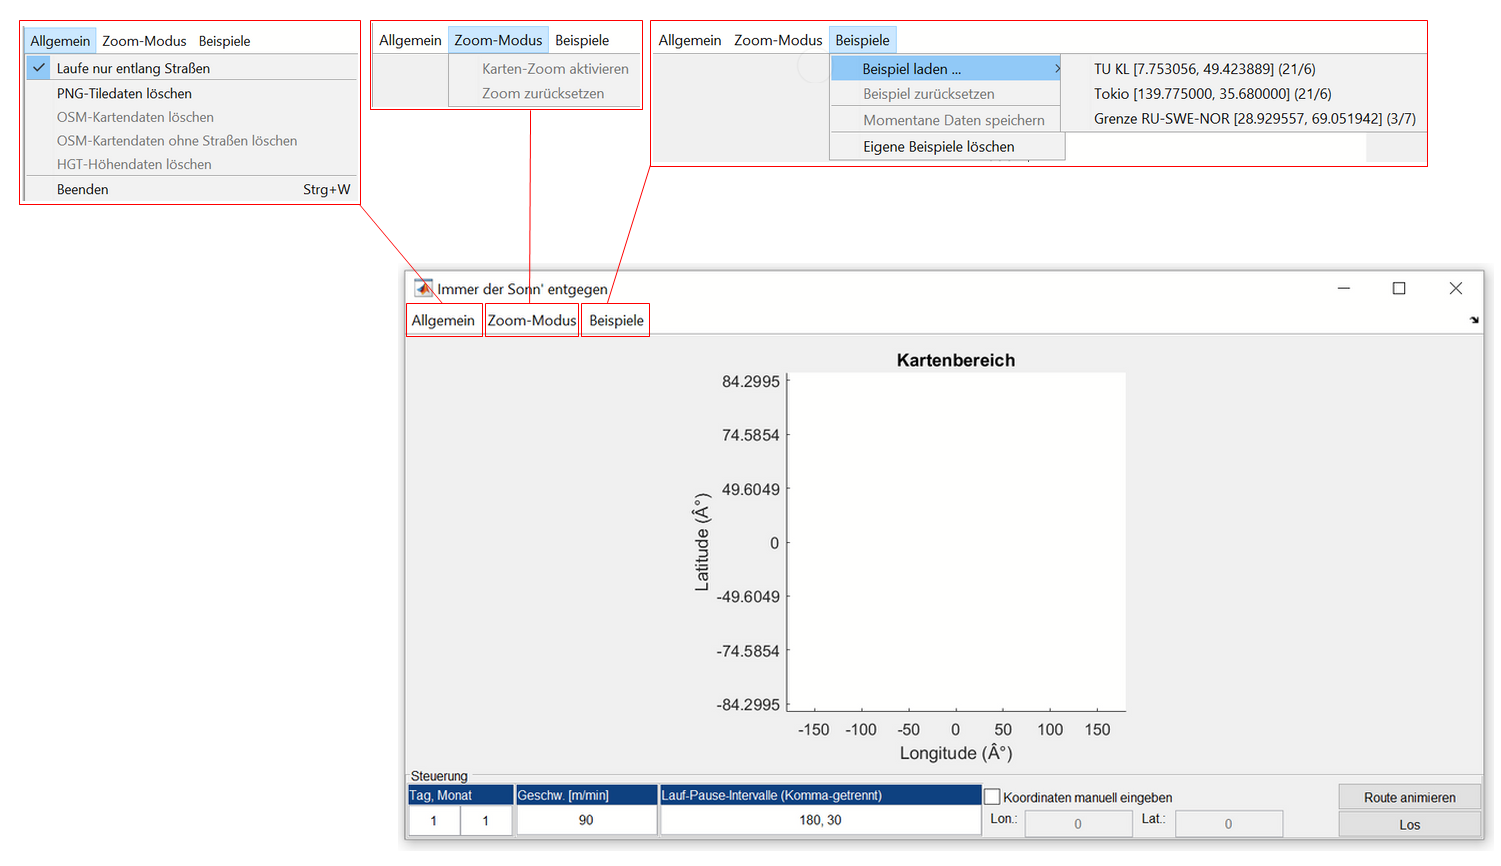
\includegraphics[width=1\textwidth]{images/gui.png}
    \caption{Grafische Benutzeroberfläche}
    \label{fig:GUI}
\end{figure}

\section{Ausblick und weitere mögliche Fragestellungen}

Von Beginn an hatten wir uns als Ziel gesetzt, das Gedankenspiel \enquote{Immer der Sonn'
entgegen} anhand von realen Daten und Gegebenheiten zu modellieren. Dies ist uns sowohl
mit der Fortbewegung auf Straßen und Wegen, als auch im freien Gelände gelungen.

Darüber hinaus haben wir uns damit beschäftigt, für welche weitere möglichen Modelle und
Ansprüche unser Modell die Grundlagen bilden könnte. Zum einen kann man stets beide
Laufmodelle im Hinblick darauf abändern, wie vorausschauend und intelligent sich der
Laufende verhalten soll. Zum anderen besteht die Möglichkeit sich statt an der Sonne an
einem anderen Planeten zu orientieren, beispielsweise dem Mond oder in Richtung eines
beliebigen Punktes oder Ortes zu laufen oder einer völlig variablen Raumkurve zu folgen.

Ebenso wäre es interessant, das Programm mobiler zu gestalten und GPS-Daten
miteinzubeziehen. Dies könnte die reale Durchführung ermöglichen, indem dem Nutzer stets
anhand seiner aktuellen Position die bestmögliche Route angezeigt wird.

Dies zeigt, dass mit unserem Modell bei weitem noch nicht alle Möglichkeiten ausgeschöpft
sind und es noch viele weitere interessante Fragestellungen existieren, welchen man sich
widmen könnte.

\begin{thebibliography}{3}
    \bibitem{wp:tobler}
        Wikipedia.
        \emph{Tobler's hiking function},
        \url{https://en.wikipedia.org/w/index.php?title=Tobler%27s_hiking_function&oldid=766415196}.
        Aufgerufen am 3.\ März 2017.
\end{thebibliography}

% Sollen wir das in dieses Dokument packen?
\appendix
\section{Verwendung unserer Skripte und Funktionen}
In diesem Anhang wollen wir noch alle von uns geschriebenen Funktionen und Skripte
auflisten und kurz erläutern, um -- sofern nicht aus der Namensgebung ersichtlich -- die
Einarbeit zur Benutzung zu erläutern.

\begin{description}[leftmargin=1em]
\item[Funktionen] werden in der finalen Version nicht mehr selbst ausgeführt, sondern von
    den entsprechenden Skripten und der grafischen Oberfläche.
    \begin{description}[format=\texttt,leftmargin=0em]
    \item[adjacencyMatrix.m] Berechnet aus gegebenem \verb|parsed_osm|-Struct die
        Adjazenzmatrix des ungerichteten Graphen, der das Straßennetzwerk repräsentiert.
    \item[day.m] Rechnet Tag und Monat in Tag des Jahres um, zum Beispiel: 1. Januar
        $\mapsto$ 1, 31. Dezember $\mapsto$ 365.
    \item[earth\_follow\_elev.m] Berechnet aus Startposition, Laufgeschwindigkeit und Datum
        die Laufroute auf einer Hindernis-losen Erde unter Berücksichtigung der Höhe.
    \item[earth\_path.m] Berechnet entweder mit unserem einfachen Sonnenmodell oder mithilfe
        der \textsc{Matlab}-Funktion \verb|SunAzEl| die nächste Position in Richtung
        Sonne in Abhängigkeit der Zeit.
    \end{description}
\item[Skripte] $ $
    \begin{description}[format=\texttt]
    \item[test]
    \end{description}
\end{description}

% Als Abschluss
Alle von uns selbst geschriebenen Skripte und Funktionen sowie die Dateien der gehaltenen
Vorstellungen sind unter \url{https://github.com/bendooru/modellier-seminar} verfügbar.

\end{document}
